\subsection{Orthographic Camera}

\begin{frame}{Orthographic Camera}
  \begin{columns}
    \begin{column}{0.5\textwidth}
      \begin{mathbox}{Orthographic Projection}
        \footnotesize
        Rays are all parallel to a specific direction, the camera's view direction $\mathbf{w}$.
        It is called orthographic projection because rays are orthogonal to the image plane.
        \only<2->{
          \begin{itemize}
            \item \textbf{No perspective distortion} \\
              Object appear the same size regardless of distance.
          \end{itemize}
        }
        \only<3->{
          \textbf{Ray Generation:}
          \begin{align*}
            \mathbf{R_o} & = \mathbf{pixel}                \\
            \mathbf{R_d} & = \mathbf{w}
          \end{align*}
        }
      \end{mathbox}
    \end{column}
    \begin{column}{0.5\textwidth}
      \begin{tikzpicture}[scale=0.5]
        \tikzset{
          screen/.style={fill=blue!10, draw=blue!50, opacity=0.8}
        }
        \coordinate (w) at (7, 0, 0);
        \coordinate (eye) at (0, 0, 0);
        \node[eye] (eye) at (0,0,0) {\faIcon{eye}};
        \draw[AccentColor, fill=AccentColor!30] (7.5, -1, 3) -- (6.25, 2.25, -3) -- (11.5, -2, 4) -- cycle;
        \node[below] at (8,-3,0) {\scriptsize \textcolor{AccentColor}{Object}};

        \begin{scope}[canvas is zy plane at x=0]
          \draw[fill=PrimaryColor!30] (-3,-3) rectangle (3,3);
          \node at (eye) {\faIcon{camera}};
        \end{scope}

        \node[above] at (3.5,4,0) {\scriptsize Screen};
        \begin{scope}[canvas is zy plane at x=3.5]
          \fill[screen] (-3,-3) rectangle (3,3);
          \foreach \x in {-3,-2,...,3} {
            \draw[gray!60, thin] (\x,-3) -- (\x,3);
          }
          \foreach \z in {-3,-2,...,3} {
            \draw[gray!60, thin] (-3,\z) -- (3,\z);
          }
          \foreach \x in {-2.5,-1.5,...,2.5} {
            \foreach \z in {-2.5,-1.5,...,2.5} {
              \fill[red!40] (\x, \z) circle (2pt);
              \draw[ray, thin, opacity=0.3] ($(\x,\z)-(w)$) -- ($(\x,\z)+(w)$);
            }
          }
          \only<2->{
            \draw[AccentColor, fill=AccentColor!30, opacity=0.7] (-2.5,2.5) -- (-1.5,-2.5) -- (2.5,-2.5) -- cycle;
          }
        \end{scope}
        \draw[ray, thick, opacity=0.9] (0, -2.5, 0.5) -- (8, -2.5, 0.5);
        \draw[ray, thick, opacity=0.9] (0, 2.5, -2.5) -- (6.5, 2.5, -2.5);
      \end{tikzpicture}
    \end{column}
  \end{columns}

  \only<4->{
    \begin{conceptbox}{Applications}
      \footnotesize
      \textbf{Technical drawings}, \textbf{CAD software}, \textbf{2D games}, architectural visualization
    \end{conceptbox}
  }
\end{frame}

\begin{frame}{Perspective vs Orthographic}
  \begin{center}
    \begin{tikzpicture}[scale=0.8]
      % Perspective
      \node at (-5, 0) {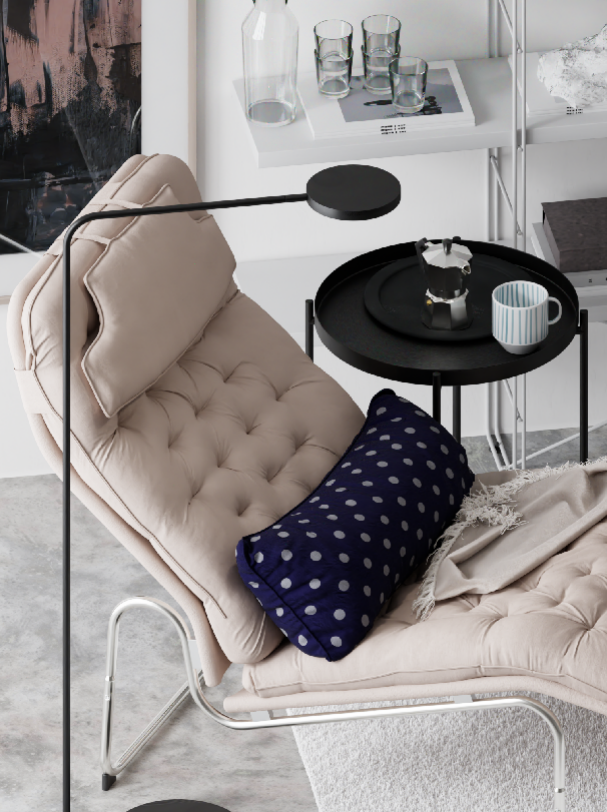
\includegraphics[width=4cm]{images/ortho.png}};
      \node at (3, 0) {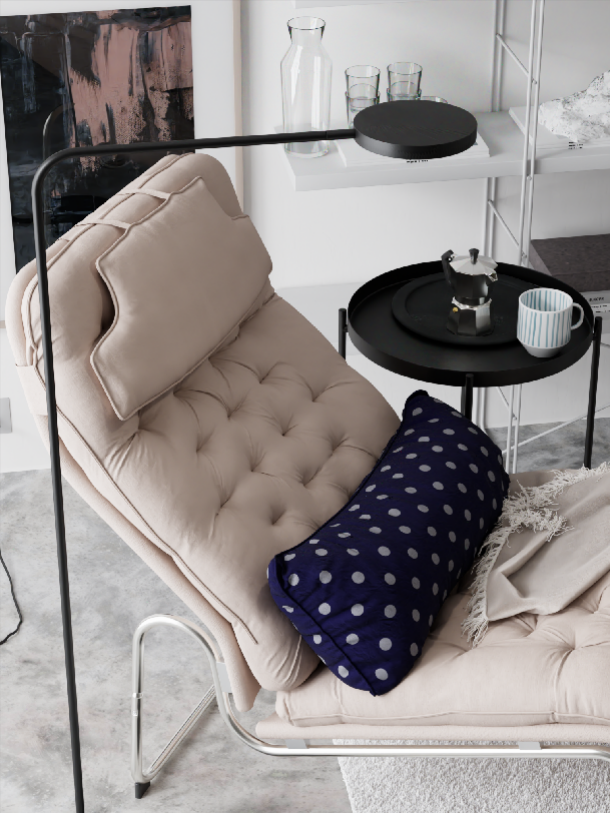
\includegraphics[width=4cm]{images/persp.png}};
    \end{tikzpicture}
  \end{center}
  \vspace*{-0.3cm}
  \begin{columns}
    \footnotesize
    \begin{column}{0.5\textwidth}
      \begin{raybox}{Perspective}
        \begin{itemize}
          \item Natural/realistic scenes
          \item Depth perception
          \item $\text{Size} \propto \frac{1}{\text{distance}}$
        \end{itemize}
      \end{raybox}
    \end{column}
    \begin{column}{0.5\textwidth}
      \begin{raybox}{Orthographic}
        \begin{itemize}
          \item CAD/Engineering
          \item Precise measurements
          \item $\text{Size} = \text{constant}$
        \end{itemize}
      \end{raybox}
    \end{column}
  \end{columns}
\end{frame}
